\subsection{Nieuwsbrief}
\pvelist{ \pve{4.25} }

De module ProRail Newsletter maakt gebruik van Drupal webforms voor het aanbieden 
van in- en uitschrijfformulieren voor nieuwsbrieven. Elke nieuwsbrief heeft 
\'{e}\'{e}n aanmeldformulier en \'{e}\'{e}n afmeldformulier. Aanmeldingen zijn 
eenvoudigweg inzendingen van de aanmeldformulieren. Er wordt niet voorzien in een 
koppeling naar een backendsysteem voor verzending, aanmeldingen dienen handmatig 
gedownload te worden als CSV-bestand (zie sectie \ref{sec:inzienaanmeldingen}). 
De module vult de webformulieren op twee belangrijke punten aan:

\begin{itemize}
\item Er wordt per aanmelding een uniek \emph{token} (een tekenreeks van 
willekeurige tekens) aangemaakt, dat meegestuurd moet worden in de 
bevestigingsemail (hiertoe moet de waarde van het tokenveld expliciet in de emailtemplate worden opgenomen) en er wordt in een bevestigingspagina voorzien, waarin 
het token verwerkt wordt en bij een juist token het veld \emph{Bevestigd} bij de aanmelding op 
\emph{Ja} wordt gezet (zie sectie \ref{sec:vereistenaanmeldformulieren}).
Op deze wijze is het niet mogelijk om een email-adres aan te melden via het 
formulier zonder toestemming van degene die werkelijk toegang heeft tot het 
email-adres. 
\item Bij het invullen van een afmeldingsformulier worden aanmeldingen voor het opgegeven 
email-adres (d.w.z. inzendingen van het bijbehorende aanmeldformulier) verwijderd.
\end{itemize}

\subsubsection{Standaard oplevering}
Bij oplevering is er als voorbeeld voorzien in twee aanmeldformulieren en een 
afmeldformulier. Het formulier \emph{Aanmelden nieuwsbrief} is ook daadwerkelijk 
geconfigureerd als aanmeldformulier, het formulier \emph{Aanmelden nieuwsbrief 
eenvoudig} is uitsluitend ter voorbeeld. Het afmeldformulier is gekoppeld aan 
het formulier \emph{Aanmelden nieuwsbrief}.
Afmeldingen kunnen, maar hoeven niet bekeken te worden; ze worden automatisch 
verwerkt, mits voldaan is aan de voorwaarden voor aan- en afmeldformulieren 
zoals hieronder opgesomd.  

\subsubsection{Inzien aanmeldingen}
\label{sec:inzienaanmeldingen}
Als voorbeeld bekijken we hoe de aanmeldingen voor de nieuwsbrief van het 
formulier \emph{Aanmelden nieuwsbrief} ingezien kunnen worden (dit is standaard webform-functionaliteit 
en werkt dus ook voor willekeurige andere webformulieren).

1. Zoek het formulier, bijvoorbeeld via de tab Webformulieren onder Inhoud
\begin{center}
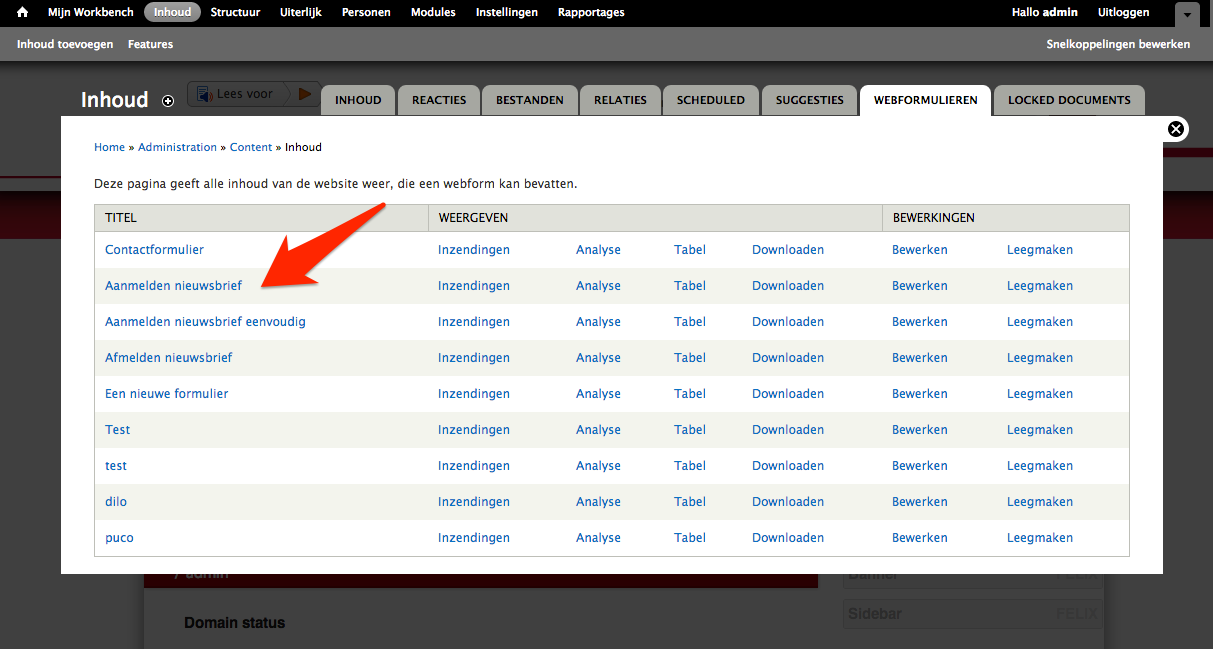
\includegraphics[width=\textwidth]{img/nieuwsbrief/form_aanmelden_nieuwsbrief.png}
\end{center}

2. Klik op de link Tabel
\begin{center}
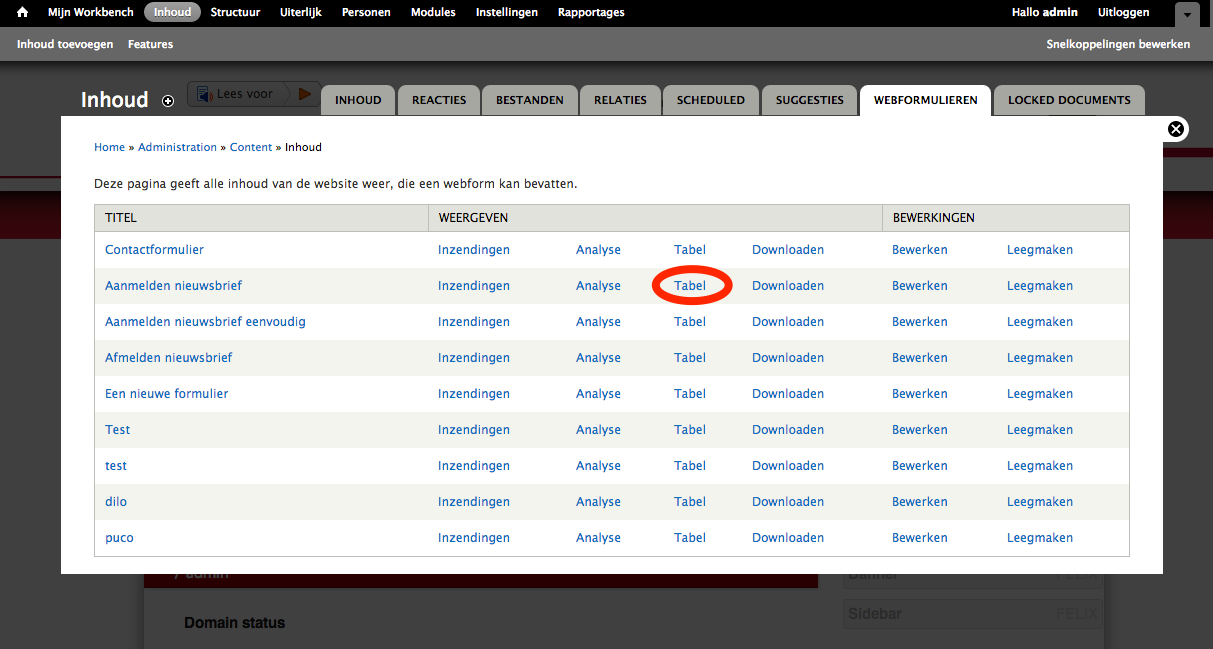
\includegraphics[width=\textwidth]{img/nieuwsbrief/aanmelden_nieuwsbrief_tabellink.png}
\end{center}

3. Een tabel met inzendingen verschijnt.
\begin{center}
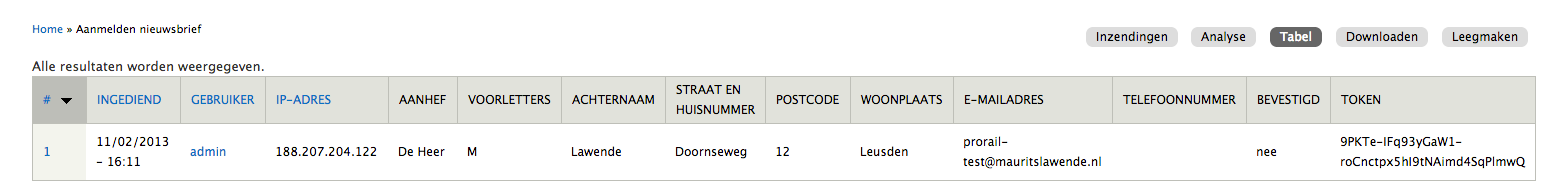
\includegraphics[width=\textwidth]{img/nieuwsbrief/aanmelden_nieuwsbrief_inzendingen.png}
\end{center}

4. De inzendingen kunnen gedownload worden als CSV-bestand op de link Download
\begin{center}
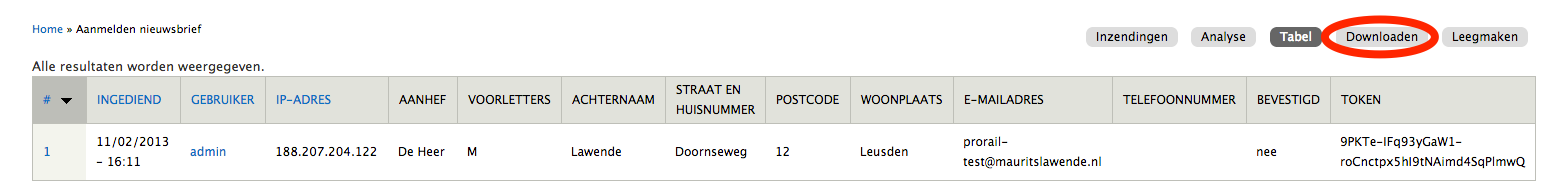
\includegraphics[width=\textwidth]{img/nieuwsbrief/aanmelden_nieuwsbrief_download.png}
\end{center}

Op dit scherm zijn een aantal instellingen mogelijk met bestrekking tot het te 
genereren export-bestand, zoals het scheidingsteken tussen waardes, welke waardes 
ge\"{e}xporteerd moeten worden en welke inzendingen gedownload moeten worden, zoals 
alleen nieuwe inzendingen, alle inzendingen, of een specifiek aantal inzendingen.

\textbf{Let op:} De download bevat alle aanmeldingen, inclusief de 
onbevestigde aanmeldingen. Het is dus bij verdere verwerking van het 
export-bestand van belang dat onbevestigde aanmeldingen worden uitgefilterd 
(dat zijn dus de aanmeldingen waarbij de kolom \emph{Bevestigd} niet op 
\emph{ja} staat).

N.b. Op het download-scherm kan gekozen worden voor het bestandsformaat 
\emph{Microsoft Excel}. Deze optie kan beter niet gebruikt worden, want de enige 
aanpassing die aan het gegenereerde bestand wordt gedaan is het veranderen van de 
bestandsnaamextensie in 
xls. De inhoud van het bestand blijft gelijk, waardoor het geen valide XLS-bestand is.

\subsubsection{Vereisten aanmeldformulieren}
\label{sec:vereistenaanmeldformulieren}
Aanmeldformulieren kunnen als normale webformulieren worden aangemaakt, mits ze aan 
een aantal eisen voldoen (op deze vereisten is geen actieve controle bij het selecteren 
van het formulier in de beheer-interface).

\begin{itemize}
\item Een veld met de machinenaam \emph{email}, dat het aangemelde email-adres bevat. Dit dient een veld van het type \emph{email} te zijn;
\item Een \emph{verborgen} veld met de machinenaam \emph{bevestigd}. Hiervoor moet 
de instelling \emph{veilige waarde} gebruikt worden zodat de 
waarde niet van buitenaf meegestuurd kan worden door middel van een malafide inzending. 
De standaard-waarde van dit veld moet op \emph{nee} ingesteld worden (in feite 
zijn hier geen beperkingen op anders dan dat de standaard-waarde niet \emph{ja}
mag zijn, want dat is de waarde die door de module wordt ingevuld bij bevestiging van 
de inschrijving).
\item Een \emph{verborgen} veld met de machinenaam \emph{token}. Dit veld wordt gebruikt voor het opslaan 
en controleren van het aangemaakte token. 
Ook hiervoor dient de instelling \emph{veilig waarde} gebruikt te worden. De 
standaard-waarde hoeft niet ingesteld te worden.
\item Een bevestigingsemail voor de gebruiker met daarin een bevestigingslink. De 
be\-ves\-ti\-gings\-link heeft de volgende vorm:
\url{http://www.prorail.nl/nieuwsbrief/bevestigen/\%value[token]}
Het voorbeeldformulier \emph{Aanmelden nieuwsbrief} bevat ook een voorbeeld van 
de bevestigingsemail met de token op de juiste manier erin opgenomen.
\end{itemize}

Naast deze velden kunnen eventueel andere velden naar keuze worden toegevoegd. Zo 
heeft het standaard opgeleverde aanmeldformulier velden voor postadres-gegevens. 
Aangeraden wordt om zo min mogelijk informatie van de gebruiker te vragen, zodat 
de drempel om voor een nieuwsbrief aan te melden zo laag mogelijk is.

\begin{figure}[p]
\centering
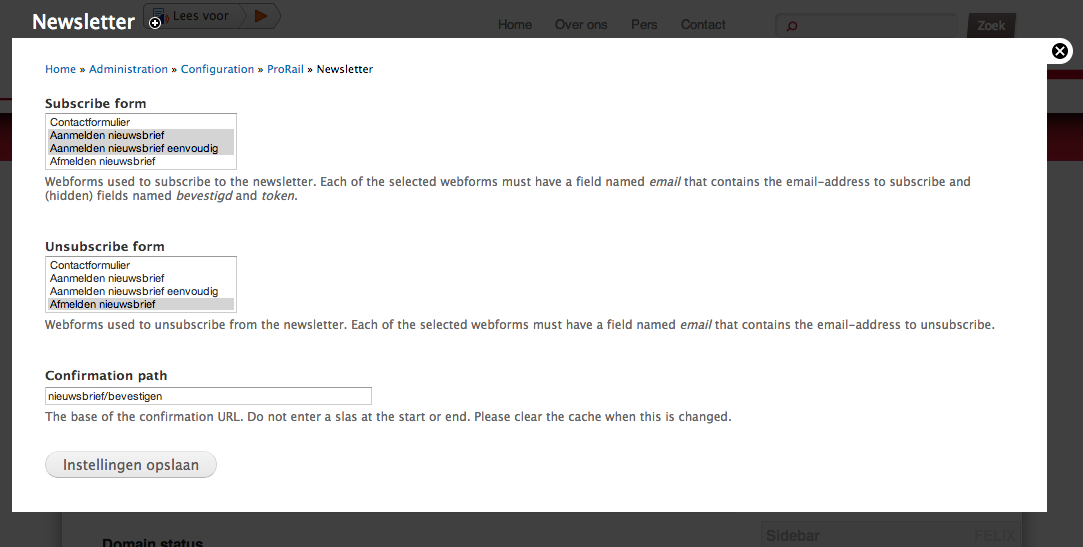
\includegraphics[width=\textwidth]{img/nieuwsbrief/nieuwsbrief_admin.png}
\end{figure}

\subsubsection{Vereisten afmeldformulieren}
\label{sec:vereistenafmeldformulieren}
De enige vereiste voor afmeldformulieren is dat ze een veld hebben met de 
machinenaam \emph{email} van het type \emph{email}. Extra velden kunnen naar 
eigen inzicht worden toegevoegd, bijvoorbeeld velden om een reden voor afmelding 
kenbaar te maken.

\subsubsection{Beheerinterface}
De beheer-interface van de module is te vinden onder Instellingen, ProRail, 
Newsletter.
De volgende instellingen zijn te maken:

\begin{itemize}
\item Het kiezen van webformulieren die dienst doen als aanmeldformulier (let op de vereisten 
zoals vermeld in \ref{sec:vereistenaanmeldformulieren}, of e.e.a. zal niet naar 
behoren werken).
\item Per aanmeldformulier een bijbehorend afmeldformulier (let op de vereisten 
zoals vermeld in \ref{sec:vereistenafmeldformulieren}).
\item Het instellen van het bevestigings-pad, dat wil zeggen de URL die de 
bevestigingen dient te verwerken. Dit is de link die vermeld dient te worden in de 
bevestigingsemail, die verantwoordelijk is voor het verwerken van aanmeldingstokens. 
Normaal gesproken hoeft dit niet aangepast te worden.
\end{itemize}

\subsubsection{Settings}

De module is instelbaar op admin/config/prorail/newsletter. Hier zijn de volgende zaken in te stellen:

\begin{enumerate}
\item Welke formulieren gelden als inschrijfformulier. Deze formulieren dienen een veld voor het email-adres te hebben met als sleutelveld 'email' en een tweetal verborgen velden, met de keys 'bevestigd' en 'token'. 'token' wordt bij indienen gevult met een unieke string, die in de bevestigingsemail wordt opgenomen in een link waarmee de aanmelding bevestigd moet worden (zie verder). 'bevestigd' wordt op 'ja' gezet zodra deze link bezocht is.

\item Welke formulieren gelden als afmeldformulier. Een email-adres ingevuld in het formulier-element met de sleutelveld 'email' heeft tot gevolg dat inzendingen van de aanmeldformulieren met dat email-adres worden verwijderd.

\item De basis voor bevestigings-URLs. Hier wordt het aangemaakte token aan vastgeplakt. Bijvoorbeeld: "nieuwsbrief/bevestigen". Het is van belang dat de URL die in de email wordt gezet hiermee overeenkomt. (Indien dit wordt verandert moet de cache gelegd worden omdat de menu router-tabel opnieuw opgebouwd moet worden).
\end{enumerate}

Voor de bevestigingsemail wordt de normale Webforms email-voorziening gebruikt. De bevestigingstoken is daar beschikbaar als value[token]. Dit is voor de huidige aanmeldformulieren al juist ingesteld.

\subsubsection{Formulieren nieuwsbrieven}

Een ingelogde gebruiker kan het formulier invullen. Er wordt dan geen e-mail verstuurd. Wel zie je de confirmatiepagina die reguliere gebruikers ook zien, waar staat dat er een e-mail is verstuurd (let dus op: dit gebeurt niet als je als content beheerder het formulier hebt ingevuld.).

Als ingelogde gebruiker kun je ook verplichte velden overslaan.

\begin{figure}[p]
\centering
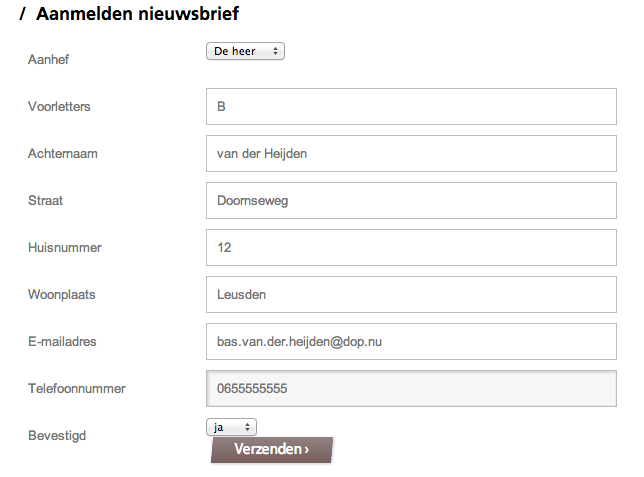
\includegraphics[width=\textwidth]{img/nieuwsbrief/nieuwsbrief_formulier.png}
\end{figure}

